% Die Arbeit besteht aus Kapiteln (chapter)
\chapter{Conceptual Design}

\section{General Design}
The goal of this thesis is to develop a system that allows generating large sets of images that are to be used for training neural networks. As this environment shall be used as a drop-in replacement for conventional methods such as taking photos and labeling those by hand, this implicates that the generated images must be of excellent quality and labeled.\\

\begin{wrapfigure}{R}{0.3\textwidth}
\centering
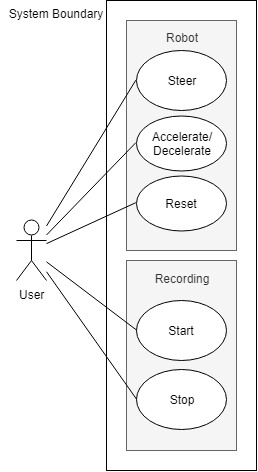
\includegraphics[width=0.3\textwidth]{tex/img/ch04/Use_Cases_04.png}
\caption{\label{fig:frog1}High-level use-cases}
\end{wrapfigure}

At its core the system features at least one virtual environment (a "scene") and a robot. it allows users to operate in one of two modes: \textit{"manual control"} lets users take control of a virtual robot and maneuver it in the virtual scene. This includes accelerating, decelerating and steering the robot as well as resetting it in case of being unable to maneuver (this may be the case when the robot is flipped or trapped between objects). This mode can be used to evaluate the usefulness (e.g. mobility) of certain robot-bodies in certain environments.\\
The second mode of operation, \textit{"automatic mode"}, allows users to let the robot travel along preconfigured paths.\\
While any of these modes is active, users can enable and disable automatic capturing of screenshots. This feature lets the system alter the scene and take screenshots from the robot's perspective in fixed intervals. is is used to create the aforementioned sets of images and does not require any user-interaction.
Figure \ref{fig:use-cases} shows the high-level use-cases described in both modes, implicating the need for at least two components: one that will be used to control a robot and one that manages taking screenshots. 

\begin{center}
\noindent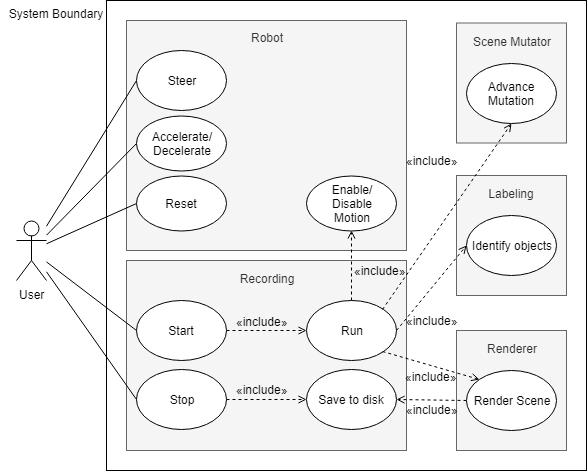
\includegraphics[width=15cm]{tex/img/ch04/Use_Cases_03.png}
\captionof{figure}{High level use cases}
\label{fig:use-cases}
\end{center}

\section{Frontend: Game Engine}

\subsection{TBD}

\subsubsection{TBD}
 
\paragraph{TBD} TBD
\paragraph{lelelel}

\section{Backend: Renderer}